\section{Modelo del programa principal}

El sistema se estructura en tres capas bien diferenciadas que separan las
responsabilidades de cada módulo y facilitan el mantenimiento y la extensibilidad
del proyecto.

\begin{itemize}
  \item \textbf{Capa de modelos.} Contiene la clase \texttt{Gramatica}, que representa
    de forma abstracta una gramática libre de contexto: almacena los conjuntos de
    terminales y no terminales, el símbolo inicial y el diccionario de producciones.

  \item \textbf{Capa de persistencia.} Agrupa tres módulos independientes:
    \texttt{lector\_archivo.py}, encargado de parsear el archivo \texttt{.txt} y
    construir el objeto \texttt{Gramatica}; \texttt{algoritmo\_primeros.py}, que
    calcula los conjuntos PRIMERO mediante iteración de punto fijo; y
    \texttt{algoritmo\_siguientes.py}, que calcula los conjuntos SIGUIENTE con la
    misma estrategia.

  \item \textbf{Capa de presentación.} Contiene los módulos de interfaz gráfica
    construidos con Tkinter: \texttt{estilos.py} define la paleta visual;
    \texttt{tabla\_base.py} y \texttt{tabla\_conjuntos.py} implementan los widgets
    de tabla reutilizables; \texttt{ventana\_primeros\_siguientes.py} presenta los
    resultados en pestañas; e \texttt{interfaz.py} actúa como punto de entrada
    de la aplicación.
\end{itemize}

\vspace{0.6cm}

\begin{figure}[h]
  \centering
  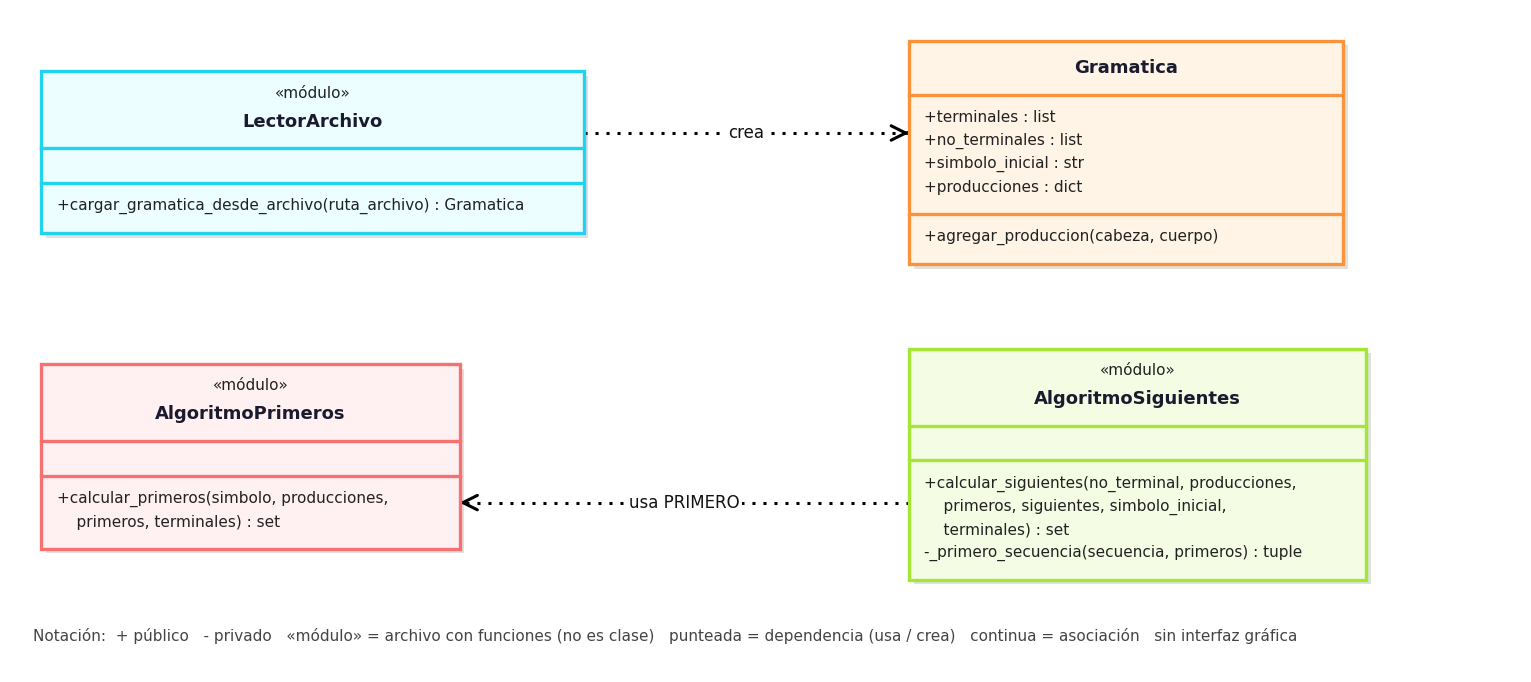
\includegraphics[width=0.92\textwidth]{imagenes/modelo_programa_principal.png}
  \caption{Modelo del programa principal \textemdash{} arquitectura en capas del sistema.}
\end{figure}
